\chapter{自发超对称破缺与第一个\texorpdfstring{\(SU(5)\)}{SU(5)}多重态}

\lectureoverview{对称性破缺在这里首次表现为关于谱的一个可见事实：旋转不变的原子具有简并的角动量能级，而磁场将它们分裂。铁磁体随后教给我们更微妙的教训：方程可能保留一种真空并不具有的对称性。无隙磁振子、条件\(J|0\rangle\neq0\)以及非零序参量是同一现象的三种描述。我们将这一模式带入手征超对称场论，通过消去辅助场\(F\)导出标量势\(V=|W'|^2\)，并区分超对称真空与\(F\)破缺真空。由此得到的真空能、玻色子--费米子分裂、戈德斯通微子、隐藏部门以及超希格斯机制完成了超对称的讨论。最后一部分改变主题并开启大统一：\(SU(3)\times SU(2)\times U(1)\)以分块方式嵌入\(SU(5)\)，其第一个物质多重态将一个轻子二重态与三个反下夸克结合在一起。}

\section{谱记得它的对称性}

从原子开始，其目的并不仅仅是复习初等量子力学。能级与粒子质量是同一种谱数据。如果一种对称性迫使原子能级重合，那么它的破缺就能分裂这些能级；在场论中，相应的陈述是粒子多重态的成员可以获得不同的质量。

设一个原子态具有总角动量\(j\)，其中包含自旋与轨道两方面的贡献。相对于任意选定的轴，
\begin{equation}
J_z|j,m\rangle=m\hbar|j,m\rangle,
\qquad
m=-j,-j+1,\ldots,j,
\end{equation}
因此有\(2j+1\)个态。教科书中熟悉的箭头不应被理解为角动量矢量真的只有\(2j+1\)个可能的空间方向。被量子化的是它沿所选轴的分量。

在空的、旋转不变的空间中，没有物理理由偏好那个轴。旋转会混合自旋为\(j\)的多重态内的各个态，而哈密顿量的不变性意味着
\begin{equation}
[H,\mathbf J]=0,
\qquad
E_{j,-j}=E_{j,-j+1}=\cdots=E_{j,j}.
\label{eq:l9-degeneracy}
\end{equation}

\begin{classroomqa}
\audiencequestion{什么对称性表明旋转整个原子不能改变其能量？\lecturetimestamp{00:05:53}}
\lecturerresponse{旋转对称性。由于旋转将角动量的一个取向变为另一个取向而不改变物理系统，所有\(2j+1\)个态都具有相同的能量。}
\end{classroomqa}

现在施加磁场\(\mathbf B=B\hat{\mathbf z}\)。相互作用
\begin{equation}
H_B=-\boldsymbol{\mu}\cdot\mathbf B
\end{equation}
区分了平行于磁场的分量。概略地说，
\begin{equation}
\Delta E_m\propto mB.
\label{eq:l9-zeeman}
\end{equation}
在弱磁场下，具有不同\(m\)的能级线性分离，而它们之间的跃迁使谱线分裂。

\begin{classroomqa}
\audiencequestion{原子能级在磁场中的分裂叫什么？\lecturetimestamp{00:07:13}}
\lecturerresponse{塞曼效应。它是整个讨论的原型：由对称性造成简并的能级，在背景破坏该对称性时发生分离。}
\end{classroomqa}

\begin{center}
\begin{tikzpicture}[x=1.05cm,y=0.75cm,>=Latex]
  \draw[thick] (-3,0) -- (-1,0);
  \node[left] at (-3,0) {\(B=0\)};
  \foreach \y/\m in {-1.2/-1,-0.4/0,0.4/1,1.2/2} {
    \draw[thick,teal!70!black] (1,\y) -- (3,\y);
    \node[right] at (3,\y) {\(m=\m\)};
  }
  \draw[->,thick] (-0.5,0) -- (0.6,0);
  \node[above] at (0.05,0) {\(\mathbf B\neq0\)};
\end{tikzpicture}
\end{center}

\section{铁磁体：对称的定律，不对称的真空}

铁磁体的一个简单微观图像为每个格点赋予一个小磁矩。如果相邻磁矩通过彼此平行而降低能量，则低温相是铁磁性的。如果反平行排列更受偏好，结果就是反铁磁性的。强烈的热涨落或量子涨落反而可能抹去任何净磁化。

假设一个铁磁体充满整个世界，并稳定到一个均匀排列的状态。它的内部磁场会像外加磁场一样分裂原子的能级。然而有一个决定性的区别。底层的相互作用并不偏好北、东或任何其他方向。每一个均匀旋转后的构型都具有相同的能量：
\begin{equation}
\mathbf M(\mathbf x)=M_0\hat{\mathbf n},
\qquad
\hat{\mathbf n}\in S^2.
\label{eq:l9-ferromagnetic-vacua}
\end{equation}
方程是旋转不变的，但一个实际的基态选择了一个\(\hat{\mathbf n}\)。这是自发对称性破缺，而非明显对称性破缺。

由这种介质的激发所构成的居民无法抓住整个宇宙并旋转它。因此，在局部看来，所选定的方向看起来就像外加磁场一样基本。原子仍然看到相同的能级图样，其角动量沿\(\hat{\mathbf n}\)而非沿外部命名的\(z\)轴分解。问题在于，内部观察者如何能够发现这种表观的不对称性属于状态，而不属于定律。

\subsection{戈德斯通诊断法}

每个磁矩的一致旋转会从式~\eqref{eq:l9-ferromagnetic-vacua}中的一个真空移动到另一个真空，并且不消耗能量。现在改为让取向在空间中非常缓慢地变化。相邻磁矩于是相互拉扯，这种畸变以自旋波的形式传播，其量子是磁振子。当波长趋于无穷大时，该构型趋近于一致旋转，因此其激发能趋于零：
\begin{equation}
k=\frac{2\pi}{\lambda}\longrightarrow0
\quad\Longrightarrow\quad
E(k)\longrightarrow0.
\label{eq:l9-gapless-magnon}
\end{equation}
两个居民可以扰动附近的磁矩，让这种波穿过介质传播，并测量这一任意低的能量。这个实验揭示了自发破缺，尽管他们无法旋转整个世界。

\editorialnote{铁磁磁振子是无能隙的，但通常具有非相对论性的二次色散\(E\propto k^2\)，而不是相对论性关系\(E\propto|k|\)。讲义在物理相关的意义上使用“无质量”一词，即能隙消失。两者都是戈德斯通模。}

同样的想法适用于连续内部对称性，包括粒子物理中的规范群和味群。然而，当被破缺的对称性被规范化时，戈德斯通模不会作为独立的无质量粒子保留下来。

\begin{classroomqa}
\audiencequestion{当自发对称性破缺与规范不变性结合时会发生什么？\lecturetimestamp{00:15:56}}
\lecturerresponse{戈德斯通玻色子为规范场提供了额外的极化。规范玻色子获得质量；这就是希格斯机制，我们将在引力类比中回到它。}
\end{classroomqa}

\section{破缺的三个等价信号}

现在可以用三种相互印证的语言来描述铁磁体。

\paragraph{简并真空。}
对于每一个取向\(\hat{\mathbf n}\)，都有一个最低能量态。物理发生在这个族中被选定的某一个成员中，尽管对称性将它们全部联系起来。

\paragraph{一个不湮灭真空的生成元。}
设\(J_a\)为旋转的一个生成元。有限变换为
\begin{equation}
U(\epsilon)=e^{-i\epsilon J_a},
\end{equation}
而\(J_a|0\rangle\)正比于真空的无穷小变化，而不是整个旋转后的态。

\begin{classroomqa}
\audiencequestion{旋转对称性的生成元是什么？\lecturetimestamp{00:17:29}}
\lecturerresponse{总角动量的各分量。我们称它们为\(J_a\)，因为它们旋转态中的一切，而不仅仅是某一个原子。}
\end{classroomqa}

未破缺的生成元满足
\begin{equation}
J_a|0\rangle=0.
\label{eq:l9-unbroken-generator}
\end{equation}
破缺的生成元则给出
\begin{equation}
J_a|0\rangle\neq0.
\label{eq:l9-broken-generator}
\end{equation}

\begin{classroomqa}
\audiencequestion{如果\(J_a|0\rangle\)非零，它是否只是给出同一个真空？\lecturetimestamp{00:19:43}}
\lecturerresponse{不是。它给出所选真空与略微旋转后的真空之间的无穷小差异。在物理上，这个差异是一个波长无限长的戈德斯通激发。}
\end{classroomqa}

\begin{classroomqa}
\audiencequestion{这个无穷小旋转会改变能量吗？\lecturetimestamp{00:20:14}}
\lecturerresponse{不会。旋转后的真空与原来的真空简并，因此零动量的戈德斯通态具有零能量。}
\end{classroomqa}

用符号表示，
\begin{equation}
J_a|0\rangle
\sim
|\pi_a,\mathbf k=0\rangle,
\label{eq:l9-generator-goldstone}
\end{equation}
其中\(\pi_a\)表示与破缺生成元相关的戈德斯通模。

\paragraph{非零序参量。}
局域磁化强度\(\mathbf M(\mathbf x)\)是一个场。在温热相或量子无序相中，
\begin{equation}
\langle\mathbf M\rangle=0,
\end{equation}
真空不选择方向。在有序相中，
\begin{equation}
\langle M_i\rangle\neq0
\quad\text{for at least one component }i,
\label{eq:l9-magnetization-order}
\end{equation}
因此旋转会将那个非零分量混合到其他分量中。简并真空、破缺生成元和非零序参量是三个要带入超对称性的模式。

\section{手征多重态回顾}

最简单的四维例子包含一个复标量、一个外尔费米子和一个辅助复标量。在手征坐标中，
\begin{equation}
y^\mu=x^\mu+i\bar\theta\bar\sigma^\mu\theta,
\end{equation}
手征超场可以示意性地展开为
\begin{equation}
\Phi(y,\theta)=
\phi(y)+\sqrt2\,\theta\psi(y)+\theta^2F(y).
\label{eq:l9-chiral-expansion}
\end{equation}
讲义省略了常规因子\(\sqrt2\)；我们从这里开始将其包含进来，以使分量系数是标准的。手征超场本质上是复的：施加实条件并不被其超对称变换所保持。

超对称动能作用量为
\begin{equation}
S_{\mathrm{kin}}
=
\int d^4x\,d^4\theta\,
\Phi^\dagger\Phi.
\label{eq:l9-kahler-action}
\end{equation}
格拉斯曼积分选出
\(\theta^2\bar\theta^2\)的系数。采用mostly-minus度规，分量结果为
\begin{equation}
\mathcal L_{\mathrm{kin}}
=
\partial_\mu\phi^\ast\,\partial^\mu\phi
+i\bar\psi\bar\sigma^\mu\partial_\mu\psi
+F^\ast F.
\label{eq:l9-chiral-kinetic}
\end{equation}
前两项传播标量和费米子。最后一项没有导数，因此不传播任何粒子。

\begin{figure}[H]
\centering
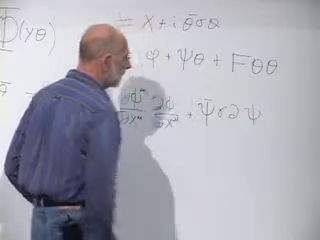
\includegraphics[width=0.76\textwidth]{lecture_09_figure_02.png}
\lectureframe{00:27:36.000}
\caption{上述手征坐标与分量展开中的标量、费米子和辅助项。}
\end{figure}

\section{\texorpdfstring{\(d^2\theta\)}{d2-theta}积分选出什么}

相互作用和质量来自一个全纯函数 \(W(\Phi)\)，即超势：
\begin{equation}
S_W
=
\int d^4x
\left[
\int d^2\theta\,W(\Phi)
+\mathrm{h.c.}
\right].
\label{eq:l9-superpotential-action}
\end{equation}
手征表达式不独立依赖于 \(\bar\theta\)，因此将其对全部四个奇坐标积分会得到零。而 \(d^2\theta\) 积分则选取其 \(\theta^2\) 分量。

在取一般函数之前，先看组合结构，令 \(W(\Phi)=\Phi^n\)。在
\begin{equation}
(\phi+\sqrt2\,\theta\psi+\theta^2F)^n,
\end{equation}
中，恰好得到两个 \(\theta\) 的方式有两种。可以选取单个 \(F\theta^2\)，或者选取两个费米子因子。

\begin{classroomqa}
\audiencequestion{有多少项包含一个选定的 \(F\theta^2\) 而其余仅为标量：\(n-1\) 还是 \(n\)？\lecturetimestamp{00:31:33}}
\lecturerresponse{共有 \(n\) 个。\(n\) 个因子中的任意一个都可以提供 \(F\theta^2\)；剩余的 \(n-1\) 个因子提供 \(\phi\)。贡献为 \(nF\phi^{n-1}\)。}
\end{classroomqa}

\begin{classroomqa}
\audiencequestion{两个因子提供两个费米子的方式有多少种？\lecturetimestamp{00:32:26}}
\lecturerresponse{共有 \(\binom n2=n(n-1)/2\) 种无序选择。格拉斯曼缩并确定了相应的 \(\psi\psi\) 项。}
\end{classroomqa}

因此，按照讲义中抑制系数的记号，
\begin{equation}
\int d^2\theta\,\Phi^n+\mathrm{h.c.}
\;\leadsto\;
nF\phi^{n-1}
-\frac{n(n-1)}{2}\phi^{n-2}\psi\psi
+\mathrm{h.c.}
\label{eq:l9-power-extraction}
\end{equation}
这里显示的负号遵循标准的归一化展开和格拉斯曼约定；改变约定可以移动表观符号。

\begin{classroomqa}
\audiencequestion{完全不包含 \(\theta\) 的项 \(\phi^n\) 怎么样了？\lecturetimestamp{00:33:10}}
\lecturerresponse{它存在于乘积中，但 \(d^2\theta\) 将其丢弃。箭头意味着积分选取 \(\theta^2\) 系数；这并不是完整表达式之间的相等。}
\end{classroomqa}

\begin{figure}[H]
\centering
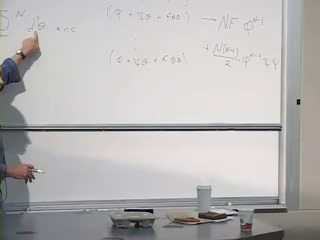
\includegraphics[width=0.82\textwidth]{lecture_09_figure_03.png}
\lectureframe{00:33:38.000}
\caption{重复的超场因子以及提取而非等于它们的双 \(\theta\) 分量的蕴含箭头。}
\end{figure}

将带有任意系数的幂次求和，把组合因子转化为导数：
\begin{equation}
\int d^2\theta\,W(\Phi)+\mathrm{h.c.}
\;\leadsto\;
F W'(\phi)
-\frac12 W''(\phi)\psi\psi
+\mathrm{h.c.}
\label{eq:l9-W-components}
\end{equation}

\begin{classroomqa}
\audiencequestion{为什么费米子项包含 \(\phi^{n-2}\)，而不是 \(\phi^{n-1}\)？\lecturetimestamp{00:36:32}}
\lecturerresponse{两个因子已经提供了费米子，剩下 \(n-2\) 个标量因子。系数是二阶导数 \(W''(\phi)\) 的一半。}
\end{classroomqa}

费米子项很重要：当 \(W''\) 为常数时它给出质量，当 \(W''\) 依赖于 \(\phi\) 时它给出汤川相互作用。然而对于真空分析，辅助项 \(FW'\) 携带直接的信息。

\section{消去辅助场}

收集包含 \(F\) 的项：
\begin{equation}
\mathcal L_F
=
F^\ast F
+F W'(\phi)
+F^\ast \overline{W'(\phi)}.
\label{eq:l9-LF}
\end{equation}
由于没有 \(\partial_\mu F\)，完整的欧拉--拉格朗日方程
\begin{equation}
\partial_\mu
\frac{\partial\mathcal L}{\partial(\partial_\mu F)}
-
\frac{\partial\mathcal L}{\partial F}
=0
\end{equation}
立即约化为一个代数方程。将 \(F\) 和 \(F^\ast\) 视为独立变量给出
\begin{align}
\frac{\partial\mathcal L_F}{\partial F}
&=F^\ast+W'(\phi)=0,
&
\frac{\partial\mathcal L_F}{\partial F^\ast}
&=F+\overline{W'(\phi)}=0,
\label{eq:l9-F-eom}
\end{align}
从而
\begin{equation}
F^\ast=-W'(\phi),
\qquad
F=-\overline{W'(\phi)}.
\label{eq:l9-F-solution}
\end{equation}

\begin{figure}[H]
\centering
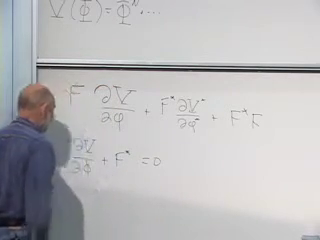
\includegraphics[width=0.82\textwidth]{lecture_09_figure_04.png}
\lectureframe{00:39:40.000}
\caption{完整的辅助场表达式及其代数运动方程，在黑板上的遮挡被清除后可以一起看到。}
\end{figure}

\begin{classroomqa}
\audiencequestion{该导数应该对 \(\phi\) 求，而不是对黑板上写的共轭场求吗？\lecturetimestamp{00:41:21}}
\lecturerresponse{是的。这一修正恢复了式~\eqref{eq:l9-F-eom}中的共轭对：\(F^\ast=-W'(\phi)\) 和 \(F=-\overline{W'(\phi)}\)。}
\end{classroomqa}

代入式~\eqref{eq:l9-LF}给出
\begin{equation}
\mathcal L_F\big|_{\mathrm{on\ shell}}
=-|W'(\phi)|^2.
\end{equation}
由于标量拉格朗日量具有动能减势能的形式，普通的标量势为
\begin{equation}
\boxed{V(\phi,\phi^\ast)=|W'(\phi)|^2\ge0.}
\label{eq:l9-F-potential}
\end{equation}
这个 \(V\) 不是超势。我们用 \(W\) 表示全纯超空间函数，用 \(V\) 表示普通势能。

\subsection{两个直接例子}

采用精确的常规归一化，
\begin{equation}
\begin{gathered}
W(\Phi)=\frac12m\Phi^2,\\
W'(\phi)=m\phi,
\qquad V=|m|^2|\phi|^2.
\end{gathered}
\label{eq:l9-quadratic-W}
\end{equation}
同一项给出费米子质量
\(-\tfrac12m\psi\psi+\mathrm{h.c.}\)，因此在超对称破缺之前标量质量和费米子质量一致。

对于
\begin{equation}
W(\Phi)=\frac{g}{3}\Phi^3,
\end{equation}
得到
\begin{equation}
\begin{gathered}
W'(\phi)=g\phi^2,
\qquad V=|g|^2|\phi|^4,\\
\mathcal L_{\mathrm{Yukawa}}
=-g\phi\psi\psi+\mathrm{h.c.}
\end{gathered}
\label{eq:l9-cubic-W}
\end{equation}
四标量顶点描述双标量散射，而汤川项是它的超对称伴随项。

\section{两类真空}

真空是 \(V\) 最小值处的常数场构型；其导数项为零。由于式~\eqref{eq:l9-F-potential}非负，有两种可能的情况。

\subsection{零能最小值}

如果某个 \(\phi_0\) 满足
\begin{equation}
W'(\phi_0)=0,
\end{equation}
那么
\begin{equation}
V(\phi_0)=0,
\qquad
\langle F\rangle=0.
\label{eq:l9-unbroken-F}
\end{equation}
真空是超对称的。这类似于磁化强度为零：没有任何辅助分量选出一个超空间方向。

\subsection{被抬升的最小值}

如果方程
\begin{equation}
W'(\phi)=0
\label{eq:l9-F-flatness}
\end{equation}
在最小值处没有同时解，那么
\begin{equation}
V_{\min}>0,
\qquad
\langle F\rangle\neq0,
\label{eq:l9-broken-F}
\end{equation}
并且超对称自发破缺。作用量仍然保持超对称；其最低能量态则不然。

\begin{figure}[H]
\centering
\includegraphics[width=0.88\textwidth]{lecture_09_figure_05.png}
\lectureframe{00:52:09.960}
\caption{黑板始终展示着正势、\(F\)方程以及真空条件，同时区分对称的方程与非对称的解。}
\end{figure}

序参量的陈述可以通过费米子变换精确表述：
\begin{equation}
\delta\psi_\alpha
=
i\sqrt2
(\sigma^\mu\bar\epsilon)_\alpha\partial_\mu\phi
+\sqrt2\,\epsilon_\alpha F.
\label{eq:l9-fermion-transformation}
\end{equation}
对于均匀真空，导数项消失。如果
\(\langle F\rangle\neq0\)，超对称将费米子平移一个非零常数，因此真空不可能不变。\editorialnote{方程~\eqref{eq:l9-fermion-transformation}是标准的分量形式，它明确表达了讲座中的陈述：超场分量相互旋转。}

同样的结论也可由超代数得出。在静止系中，
\begin{equation}
\{Q_\alpha,Q_{\dot\alpha}^\dagger\}
=2\sigma^0_{\alpha\dot\alpha}H.
\end{equation}
取真空期望值将其能量表示为超荷作用于真空的模方之和：
\begin{equation}
E_0\ge0,
\qquad
E_0=0
\ \Longleftrightarrow\
Q_\alpha|0\rangle
=Q_{\dot\alpha}^\dagger|0\rangle=0.
\label{eq:l9-algebra-vacuum-energy}
\end{equation}
因此，正的真空能量与自发超对称破缺是同一个刚性超对称陈述的两面。

\begin{center}
\begin{tikzpicture}[x=1.2cm,y=1.0cm,>=Latex]
  \draw[->] (-3,0) -- (-0.2,0) node[right] {\(\phi\)};
  \draw[->] (-2.8,-0.15) -- (-2.8,2.1) node[above] {\(V\)};
  \draw[thick,teal!75!black,domain=-2.5:-0.5,samples=60]
    plot (\x,{0.65*(\x+1.5)^2});
  \fill (-1.5,0) circle (2pt);
  \node[below] at (-1.5,0) {\(F=0\)};
  \draw[->] (0.4,0) -- (3.2,0) node[right] {\(\phi\)};
  \draw[->] (0.6,-0.15) -- (0.6,2.1) node[above] {\(V\)};
  \draw[thick,orange!85!black,domain=0.9:2.9,samples=60]
    plot (\x,{0.55*(\x-1.9)^2+0.65});
  \fill (1.9,0.65) circle (2pt);
  \draw[dashed] (0.6,0.65) -- (1.9,0.65);
  \node[below] at (1.9,0.65) {\(F\neq0\)};
\end{tikzpicture}
\end{center}

\editorialnote{一个最小的例子是\(W=f\Phi\)，对此\(W'=f\)永不消失，且\(V=|f|^2\)。这个单场例子具有平坦的标量方向；现实的稳定\(F\)项破缺通常用多个手征场来实现，如O'Raifeartaigh型隐藏部门。}

\section{破缺的超对称产生什么}

\subsection{质量劈裂}

铁磁类比现在又变成了谱学的。一个弱的内部磁场将原子能级分开，而不破坏原子的同一性。类似地，一个弱传递的超对称破缺序参量将原本处于同一超多重态中的玻色子和费米子分开。

\begin{classroomqa}
\audiencequestion{哪些粒子被超对称相互旋转，从而在真空破缺它时失去质量简并？\lecturetimestamp{00:51:40}}
\lecturerresponse{玻色子和费米子。一旦态不再尊重联系它们的变换，它们的质量就不必保持相等。}
\end{classroomqa}

劈裂并非由孤立的\(\langle F\rangle\)产生；它取决于将破缺传递给可见场的耦合。如果这些耦合很弱，可见粒子仍可辨认，且劈裂与大一统或普朗克尺度相比很小。如果它们很强，类比将是一个被巨大磁场扭曲得面目全非的长条形原子。

\subsection{戈德斯通费米子}

对于普通的破缺生成元，\(J|0\rangle\)给出一个玻色型戈德斯通态。超荷是费米型的，将玻色态变为费米态。由于真空被算作玻色型，破缺的超荷产生一个费米型零能态：
\begin{equation}
Q_\alpha|0\rangle
\sim
|\widetilde G_\alpha,\mathbf k=0\rangle.
\label{eq:l9-goldstino}
\end{equation}
其传播延续是一个无质量外尔费米子，即戈德斯通费米子或戈德斯通微子。

\begin{classroomqa}
\audiencequestion{如果超对称变换不保持真空不变，它会产生什么新态？\lecturetimestamp{00:53:24}}
\lecturerresponse{一个无质量费米子。普通戈德斯通定理的模式仍然成立，但费米型生成元将玻色型真空变为戈德斯通费米子。}
\end{classroomqa}

因此，刚性自发超对称破缺有两个不可避免的特征：
\begin{equation}
\boxed{
V_{\min}>0
\qquad\text{and}\qquad
\text{a massless goldstino}.
}
\label{eq:l9-rigid-breaking-signatures}
\end{equation}

\section{隐藏部门}

将原子和铁磁体称为两个部门是有用的。铁磁体发展出序参量；原子只感受到从它传递来的场。当耦合很弱时，操纵原子几乎不会激发磁振子，也几乎无法直接接触磁性介质。此时铁磁体是隐藏的，尽管其存在可由微小的谱劈裂推断出来。

超对称模型构建使用同样的语言。隐藏部门中的额外场发展出非零的\(F\)项或\(D\)项期望值。称为传递机制的相互作用将这种破缺传递给可见部门，并为超伴侣产生软质量。弱传递解释了可见理论如何能在高得多的基本尺度下保持近似超对称，同时不表现出精确的低能玻色子--费米子简并。

这种构造并非自动成立。需要额外场、稳定的破缺真空以及受控的传递机制。这就是为什么讲座将现实的超对称破缺描述为复杂且有些做作，而不是最小模型的单一必然结果。

\section{引力改变两个特征}

\subsection{真空能量成为源}

没有引力时，将所有能量平移一个常数不会改变非引力实验。有引力时，真空能量密度作为宇宙学常数进入爱因斯坦方程。正的\(V_{\min}\)驱动加速膨胀。如果其尺度与超对称伙伴质量所需的粒子物理尺度相当，那么由此产生的曲率将比观测到的值大得不可估量。

\begin{classroomqa}
\audiencequestion{一旦把引力包括进来，正的、非零的真空能量会对世界产生什么影响？\lecturetimestamp{01:00:40}}
\lecturerresponse{它充当宇宙学常数并驱动加速膨胀。在普通的粒子物理尺度上，这种效应会大得令人无法接受。}
\end{classroomqa}

局域超对称，即超引力，会改变正平方公式。为了便于定位，标准的\(N=1\) \(F\)项势为
\begin{equation}
\begin{aligned}
V_F={}&e^{K/M_P^2}
\left(
K^{i\bar j}D_iW\,D_{\bar j}\overline W
-\frac{3|W|^2}{M_P^2}
\right),\\
D_iW={}&\partial_iW+\frac{\partial_iK}{M_P^2}W.
\end{aligned}
\label{eq:l9-sugra-potential}
\end{equation}
由于负项的存在，原则上，来自超对称破缺的正能量可以部分被抵消。剩余部分可能是一个很小的宇宙学常数。

\editorialnote{本讲有意只给出示意性的修正，并明确质疑普朗克质量的放置位置。方程~\eqref{eq:l9-sugra-potential}记录了具有Kähler势\(K\)的手征多重态的传统公式；规范\(D\)项还会增加一个非负贡献。它并未解释观测到的极小值，而这仍然是宇宙学常数问题。}

\subsection{超希格斯机制}

第二个引力效应最容易通过数极化态来理解。一个质量为自旋\(j\)的粒子在其静止系中有\(2j+1\)个自旋态。

\begin{classroomqa}
\audiencequestion{一个质量为自旋\(j\)的粒子有多少个自旋态？\lecturetimestamp{01:05:16}}
\lecturerresponse{\(2j+1\)。特别地，一个质量为自旋1的粒子有三个态，而无质量规范玻色子只有螺旋度\(+1\)和\(-1\)。}
\end{classroomqa}

这一区别是运动学的。一个有质量粒子可以被助推到静止，然后在其自旋取向保持不变的情况下被送往新的方向，因此所有投影都必须存在。一个无质量粒子不能被追上或带到静止。因此它只能携带两个极端螺旋度。

对于电弱规范场，
\begin{equation}
\underbrace{(+1,-1)}_{\text{massless vector}}
+
\underbrace{(0)}_{\text{Goldstone}}
\longrightarrow
\underbrace{(+1,0,-1)}_{\text{massive vector}}.
\label{eq:l9-higgs-count}
\end{equation}

\begin{classroomqa}
\audiencequestion{一个有质量的\(W\)或\(Z\)的纵向极化来自哪里？\lecturetimestamp{01:08:50}}
\lecturerresponse{来自Goldstone玻色子。它被规范场吸收，并补全三态的有质量自旋1表示。}
\end{classroomqa}

引力有一个无质量自旋2的引力子。它的超对称伙伴是无质量自旋\(\tfrac32\)的引力微子。

\begin{classroomqa}
\audiencequestion{引力子的自旋是多少，因此它的超对称伙伴的自旋是多少？\lecturetimestamp{01:10:24}}
\lecturerresponse{引力子的自旋为\(2\)；费米子伙伴相差二分之一，自旋为\(3/2\)。}
\end{classroomqa}

无质量引力微子具有螺旋度\(\pm\tfrac32\)，而有质量引力微子还必须具有\(\pm\tfrac12\)。Goldstino恰好提供了那些缺失的态：
\begin{equation}
\begin{gathered}
\underbrace{\left(+\frac32,-\frac32\right)}_{\text{massless gravitino}}
\oplus
\underbrace{\left(+\frac12,-\frac12\right)}_{\text{goldstino}}\\
\Downarrow\\
\underbrace{\left(+\frac32,+\frac12,-\frac12,-\frac32\right)}_{\text{massive gravitino}}.
\end{gathered}
\label{eq:l9-super-higgs}
\end{equation}
这就是超希格斯机制。一旦超对称是局域的，Goldstino就被吸收，不再作为独立的无质量粒子出现。由此产生的引力微子以引力方式相互作用，因此相应地难以产生。

\section{转换主题：为什么是\texorpdfstring{\(SU(5)\)}{SU(5)}？}

超对称形式体系现在让位于大统一。标准模型规范群是
\begin{equation}
G_{\mathrm{SM}}
=SU(3)_c\times SU(2)_L\times U(1)_Y.
\label{eq:l9-sm-group}
\end{equation}
它的三个因子分别组织色、弱同位旋和弱超荷。统一的问题是：这个乘积是否是一个更大单群的剩余子群，从而表面上分离的粒子多重态和规范力是单一结构的组成部分。这里发展的最小候选者是\(SU(5)\)。

\subsection{群元素与生成元}

对于\(U\in SU(N)\)，
\begin{equation}
U^\dagger U=\mathbf1,
\qquad
\det U=1.
\label{eq:l9-SUN-def}
\end{equation}
第一个条件是幺正的；第二个是special的含义。将无穷小元素写为
\begin{equation}
U=\mathbf1+i\epsilon G+\mathcal O(\epsilon^2).
\label{eq:l9-infinitesimal-U}
\end{equation}
幺正性要求
\begin{equation}
G^\dagger=G,
\end{equation}
而
\begin{equation}
\det e^{i\epsilon G}
=e^{i\epsilon\operatorname{tr}G}=1
\end{equation}
要求
\begin{equation}
\operatorname{tr}G=0.
\end{equation}
因此生成元是无迹厄米矩阵。

一个\(N\times N\)厄米矩阵包含\(N^2\)个实参数：\(N\)个实对角元以及\(N(N-1)/2\)个复非对角元。无迹性去掉一个。因此
\begin{equation}
\dim SU(N)=N^2-1,
\qquad
\dim SU(5)=24.
\label{eq:l9-SU5-dimension}
\end{equation}
作为比较，\(SU(2)\)有三个Pauli生成元，而\(SU(3)\)有八个色生成元。

\section{\texorpdfstring{\(SU(5)\)}{SU(5)}内部的标准模型块}

将五维空间分成弱相互作用的二维块和色三维块：
\begin{equation}
\mathbf5=\mathbf2\oplus\mathbf3.
\end{equation}
嵌入的生成元具有如下形式
\begin{align}
T^a_L
&=
\begin{pmatrix}
\tfrac12\tau^a&0\\
0&0_{3\times3}
\end{pmatrix},
&& a=1,2,3,
\label{eq:l9-SU2-block}\\
T^A_c
&=
\begin{pmatrix}
0_{2\times2}&0\\
0&\tfrac12\lambda^A
\end{pmatrix},
&& A=1,\ldots,8.
\label{eq:l9-SU3-block}
\end{align}
泡利矩阵\(\tau^a\)生成弱\(SU(2)\)；盖尔曼矩阵\(\lambda^A\)生成色\(SU(3)\)。由于这两个块不重叠，两个子群对易。

还有一个对角生成元，在每个块内与单位矩阵成正比，因此与两者都对易。在基础表示中，一种方便的双重超荷约定是
\begin{equation}
T_Y^{(\mathbf5)}=
\operatorname{diag}
\left(
1,1,-\frac23,-\frac23,-\frac23
\right).
\label{eq:l9-hypercharge-generator}
\end{equation}
它的迹为零：
\begin{equation}
1+1-3\left(\frac23\right)=0.
\end{equation}
共轭物质表示具有相反的本征值，
\begin{equation}
Y_{\overline{\mathbf5}}
=
\operatorname{diag}
\left(
-1,-1,\frac23,\frac23,\frac23
\right),
\label{eq:l9-fivebar-hypercharge}
\end{equation}
这些就是讲义中物质列所写的值。整体符号和归一化是约定性的；这些条目采用标准模型约定
\begin{equation}
Q=T_3+\frac{Y}{2}.
\label{eq:l9-charge}
\end{equation}
方程~\eqref{eq:l9-SU2-block}--\eqref{eq:l9-hypercharge-generator}展示
\begin{equation}
SU(3)_c\times SU(2)_L\times U(1)_Y
\subset SU(5).
\end{equation}

三个弱生成元、八个色生成元和一个超荷生成元占据了\(24\)个\(SU(5)\)生成元中的\(12\)个。\editorialnote{其余十二个占据非对角的\(2\times3\)块和\(3\times2\)块。它们的规范玻色子将夸克型分量和轻子型分量相互转化；这就是后续发展中重子数和轻子数改变相互作用的结构性起源。}

\begin{classroomqa}
\audiencequestion{哪些规范粒子对应于熟悉的子群生成元？\lecturetimestamp{01:31:05}}
\lecturerresponse{八个\(SU(3)\)生成元给出八个胶子。三个\(SU(2)\)生成元给出弱规范场，它们在电弱混合后成为\(W^\pm\)以及\(Z\)-光子系统的一部分；\(U(1)\)场提供另一个中性组合。}
\end{classroomqa}

\section{左手语言中的一代}

聚焦于第一代；同样的模式对{\proseunicodefont μ}子/粲夸克/奇异夸克代和{\proseunicodefont τ}子/顶夸克/底夸克代重复出现。最经济的做法是把每个独立的Weyl场都计为左手场。右手粒子由它们的左手电荷共轭场表示：
\begin{equation}
Q_L=(u_L,d_L),\quad
L_L=(\nu_{eL},e_L),\quad
u^c_L,\quad d^c_L,\quad e^c_L.
\end{equation}
它们的重数为
\begin{equation}
\underbrace{6}_{Q_L}
+
\underbrace{2}_{L_L}
+
\underbrace{3}_{u^c_L}
+
\underbrace{3}_{d^c_L}
+
\underbrace{1}_{e^c_L}
=15.
\label{eq:l9-fifteen-fields}
\end{equation}

\editorialnote{最小标准模型不包含独立的右手中微子Weyl场，因此计数为\(15\)。仅凭这一计数并不能断言中微子是Majorana粒子。加入一个单态\(\nu^c_L\)后，场数变为\(16\)，并自然地指向\(SO(10)\)，超出当前的\(SU(5)\)构造。}

五维多重态必须把无色的弱二重态条目放在前两个位置，把有色的弱单态放在后三个位置。

\begin{classroomqa}
\audiencequestion{所提出的列包含六个场而不是五个吗？\lecturetimestamp{01:36:14}}
\lecturerresponse{不。第一遍写下的上夸克被擦除。该列是中微子、电子以及反下夸克的三个色副本：总共五个条目。}
\end{classroomqa}

这给出
\begin{equation}
\overline{\mathbf5}
=
\begin{pmatrix}
\nu_{eL}\\
e_L\\
d^c_{rL}\\
d^c_{gL}\\
d^c_{bL}
\end{pmatrix}.
\label{eq:l9-fivebar}
\end{equation}
\editorialnote{讲义最初只把它称为一个五维多重态。在标准的全左手\(SU(5)\)记号中，它的色和超荷分配表明它是共轭表示\(\overline{\mathbf5}\)。}
前两个条目在\(SU(2)_L\)下变换，但不带色。后三个条目在色下作为反三重态变换，但它们是弱单态。

\begin{classroomqa}
\audiencequestion{当每个场都写成左手场后，哪些夸克带色但不带弱\(SU(2)_L\)量子数？\lecturetimestamp{01:40:13}}
\lecturerresponse{右手夸克的电荷共轭。对于这个五分量的多重态，电荷检验选出三个反下夸克场\(d^c_{r,g,b}\)。}
\end{classroomqa}

方程~\eqref{eq:l9-fivebar}中的电荷之和为零：
\begin{equation}
0-1+\frac13+\frac13+\frac13=0.
\label{eq:l9-fivebar-charge-sum}
\end{equation}
这是必需的，因为电荷算符是\(SU(5)\)生成元的无迹组合。

\begin{classroomqa}
\audiencequestion{为什么占据三个色位置的是反下夸克，而不是反上夸克？\lecturetimestamp{01:43:38}}
\lecturerresponse{中微子和电子贡献的总电荷为\(-1\)。三个反下夸克色贡献\(+1\)，使迹为零。三个反上夸克场会有错误的总电荷。}
\end{classroomqa}

剩余的十个左手场是
\begin{equation}
Q_L\;(6)
\oplus
u^c_L\;(3)
\oplus
e^c_L\;(1),
\end{equation}
它们恰好适合反对称的二阶表示
\begin{equation}
\mathbf{10}\cong\wedge^2\mathbf5,
\qquad
\dim\wedge^2\mathbf5=\binom52=10.
\label{eq:l9-ten-preview}
\end{equation}
它们的显式放置是下一讲的任务。对每个标准模型代都有数值匹配
\begin{equation}
\overline{\mathbf5}\oplus\mathbf{10}
\end{equation}
这是\(SU(5)\)思想不只是任意重新标记的第一个引人注目的证据。

\begin{classroomqa}
\audiencequestion{如果五重态和十重态是不同的表示，这是否意味着它们的粒子不能相互作用？\lecturetimestamp{01:46:14}}
\lecturerresponse{不。群变换在每个不可约表示内部作用，因此它不会直接把五重态的一个成员旋转成十重态的一个成员。然而，这两组粒子可以通过发射和吸收共同的规范玻色子而相互作用，希格斯耦合也能连接它们的场。}
\end{classroomqa}

\section{展望}

本讲在差异极大的尺度上追踪了同一个模式。旋转不变性使原子能级简并；磁背景将它们劈裂。铁磁体产生这样的背景，同时让底层定律保持对称，而其无能隙磁振子表明不对称性存在于真空中。在手征超对称理论中，辅助场期望值扮演序参量的角色：
\begin{equation}
\begin{aligned}
\langle F\rangle=0
&\quad\Longleftrightarrow\quad
\text{unbroken supersymmetry},\\
\langle F\rangle\neq0
&\quad\Longrightarrow\quad
\text{spontaneous breaking}.
\end{aligned}
\end{equation}
在刚性超对称中，破缺的真空带有正能量，劈裂超多重态，并产生戈德斯通费米子。弱媒介作用为隐藏部门提供了动机；引力把真空能变成宇宙学问题，并把戈德斯通费米子吸收进有质量的引力微子。

收尾的\(SU(5)\)构造开启了一个新问题，而不是完成了它。无迹厄米\(5\times5\)生成元包含标准模型各块，而前五个物质场恰好按
\((\nu_e,e^-,d^c_r,d^c_g,d^c_b)\)的方式嵌入。剩下的十个则在反对称表示中等待。这一未完成的嵌入正是大统一真正开始之处。
